\documentclass[12pt,a4paper,oneside,pdftex]{report}

% The input files (tex files) are encoded with the latin-1 encoding 
% (ISO-8859-1 works). Change the latin1-option if you use UTF8 
% (at some point LaTeX did not work with UTF8, but I'm not sure
% what the current situation is) 
%\usepackage[latin1]{inputenc}
\usepackage[utf8]{inputenc}
% OT1 font encoding seems to work better than T1. Check the rendered
% PDF file to see if the fonts are encoded properly as vectors (instead
% of rendered bitmaps). You can do this by zooming very close to any letter 
% - if the letter is shown pixelated, you should change this setting 
% (try commenting out the entire line, for example).  
\usepackage[OT1]{fontenc}
% The babel package provides hyphenating instructions for LaTeX. Give
% the languages you wish to use in your thesis as options to the babel
% package (as shown below). You can remove any language you are not
% going to use.
% Examples of valid language codes: english (or USenglish), british, 
% finnish, swedish; and so on.
\usepackage[finnish,swedish,english]{babel}


% Font selection
% ------------------------------------------------------------------
% The default LaTeX font is a very good font for rendering your 
% thesis. It is a very professional font, which will always be 
% accepted. 
% If you, however, wish to spicen up your thesis, you can try out
% these font variants by uncommenting one of the following lines
% (or by finding another font package). The fonts shown here are 
% all fonts that you could use in your thesis (not too silly). 
% Changing the font causes the layouts to shift a bit; you many
% need to manually adjust some layouts. Check the warning messages
% LaTeX gives you.
% ------------------------------------------------------------------
% To find another font, check out the font catalogue from
% http://www.tug.dk/FontCatalogue/mathfonts.html
% This link points to the list of fonts that support maths, but
% that's a fairly important point for master's theses.
% ------------------------------------------------------------------
% <rant>
% Remember, there is no excuse to use Comic Sans, ever, in any
% situation! (Well, maybe in speech bubbles in comics, but there 
% are better options for those too)
% </rant>

% \usepackage{palatino}
% \usepackage{tgpagella}



% Optional packages
% ------------------------------------------------------------------
% Select those packages that you need for your thesis. You may delete
% or comment the rest.

% Natbib allows you to select the format of the bibliography references.
% The first example uses numbered citations: 
\usepackage[square,sort&compress,numbers]{natbib}
% The second example uses author-year citations.
% If you use author-year citations, change the bibliography style (below); 
% acm style does not work with author-year citations.
% Also, you should use \citet (cite in text) when you wish to refer
% to the author directly (\citet{blaablaa} said blaa blaa), and 
% \citep when you wish to refer similarly than with numbered citations
% (It has been said that blaa blaa~\citep{blaablaa}).
% \usepackage[square]{natbib}

% The alltt package provides an all-teletype environment that acts
% like verbatim but you can use LaTeX commands in it. Uncomment if 
% you want to use this environment. 
% \usepackage{alltt}

% The eurosym package provides a euro symbol. Use with \euro{}
\usepackage{eurosym} 

% Verbatim provides a standard teletype environment that renderes
% the text exactly as written in the tex file. Useful for code
% snippets (although you can also use the listings package to get
% automatic code formatting). 
\usepackage{verbatim}

% The listing package provides automatic code formatting utilities
% so that you can copy-paste code examples and have them rendered
% nicely. See the package documentation for details.
% \usepackage{listings}

% The fancuvrb package provides fancier verbatim environments 
% (you can, for example, put borders around the verbatim text area
% and so on). See package for details.
% \usepackage{fancyvrb}

% Supertabular provides a tabular environment that can span multiple 
% pages. 
%\usepackage{supertabular}
% Longtable provides a tabular environment that can span multiple 
% pages. This is used in the example acronyms file. 
\usepackage{longtable}

% The fancyhdr package allows you to set your the page headers 
% manually, and allows you to add separator lines and so on. 
% Check the package documentation. 
% \usepackage{fancyhdr}

% Subfigure package allows you to use subfigures (i.e. many subfigures
% within one figure environment). These can have different labels and
% they are numbered automatically. Check the package documentation. 
\usepackage{subfigure}

% The titlesec package can be used to alter the look of the titles 
% of sections, chapters, and so on. This example uses the ``medium'' 
% package option which sets the titles to a medium size, making them
% a bit smaller than what is the default. You can fine-tune the 
% title fonts and sizes by using the package options. See the package
% documentation.
\usepackage[medium]{titlesec}

% The TikZ package allows you to create professional technical figures.
% The learning curve is quite steep, but it is definitely worth it if 
% you wish to have really good-looking technical figures. 
\usepackage{tikz}
% You also need to specify which TikZ libraries you use
\usetikzlibrary{positioning}
\usetikzlibrary{calc}
\usetikzlibrary{arrows}
\usetikzlibrary{decorations.pathmorphing,decorations.markings}
\usetikzlibrary{shapes}
\usetikzlibrary{patterns}


% The aalto-thesis package provides typesetting instructions for the
% standard master's thesis parts (abstracts, front page, and so on)
% Load this package second-to-last, just before the hyperref package.
% Options that you can use: 
%   mydraft - renders the thesis in draft mode. 
%             Do not use for the final version. 
%   doublenumbering - [optional] number the first pages of the thesis
%                     with roman numerals (i, ii, iii, ...); and start
%                     arabic numbering (1, 2, 3, ...) only on the 
%                     first page of the first chapter
%   twoinstructors  - changes the title of instructors to plural form
%   twosupervisors  - changes the title of supervisors to plural form
\usepackage[mydraft,twosupervisors]{aalto-thesis}
%\usepackage[mydraft,doublenumbering]{aalto-thesis}
%\usepackage{aalto-thesis}


% Hyperref
% ------------------------------------------------------------------
% Hyperref creates links from URLs, for references, and creates a
% TOC in the PDF file.
% This package must be the last one you include, because it has
% compatibility issues with many other packages and it fixes
% those issues when it is loaded.   
\RequirePackage[pdftex]{hyperref}
% Setup hyperref so that links are clickable but do not look 
% different
\hypersetup{colorlinks=false,raiselinks=false,breaklinks=true}
\hypersetup{pdfborder={0 0 0}}
\hypersetup{bookmarksnumbered=true}
% The following line suggests the PDF reader that it should show the 
% first level of bookmarks opened in the hierarchical bookmark view. 
\hypersetup{bookmarksopen=true,bookmarksopenlevel=1}
% Hyperref can also set up the PDF metadata fields. These are
% set a bit later on, after the thesis setup.   


% Thesis setup
% ==================================================================
% Change these to fit your own thesis.
% \COMMAND always refers to the English version;
% \FCOMMAND refers to the Finnish version; and
% \SCOMMAND refers to the Swedish version.
% You may comment/remove those language variants that you do not use
% (but then you must not include the abstracts for that language)
% ------------------------------------------------------------------
% If you do not find the command for a text that is shown in the cover page or
% in the abstract texts, check the aalto-thesis.sty file and locate the text
% from there. 
% All the texts are configured in language-specific blocks (lots of commands
% that look like this: \renewcommand{\ATCITY}{Espoo}.
% You can just fix the texts there. Just remember to check all the language
% variants you use (they are all there in the same place). 
% ------------------------------------------------------------------
\newcommand{\TITLE}{Improving Object Classification Using Data Augmentation }
\newcommand{\SUBTITLE}{A Case Study in Application of Data Augmentation}
\newcommand{\DATE}{Jan 1 2018}

% Supervisors and instructors
% ------------------------------------------------------------------
% If you have two supervisors, write both names here, separate them with a 
% double-backslash (see below for an example)
% Also remember to add the package option ``twosupervisors'' or
% ``twoinstructors'' to the aalto-thesis package so that the titles are in
% plural.
% Example of one supervisor:
%\newcommand{\SUPERVISOR}{Professor Antti Ylä-Jääski}
%\newcommand{\FSUPERVISOR}{Professori Antti Ylä-Jääski}
%\newcommand{\SSUPERVISOR}{Professor Antti Ylä-Jääski}
% Example of twosupervisors:
\newcommand{\SUPERVISOR}{Professor Antti Ylä-Jääski\\
	Professor Pekka Perustieteilijä}
\newcommand{\FSUPERVISOR}{Professori Antti Ylä-Jääski\\
	Professori Pekka Perustieteilijä}
\newcommand{\SSUPERVISOR}{Professor Antti Ylä-Jääski\\
	Professor Pekka Perustieteilijä}

% If you have only one instructor, just write one name here
\newcommand{\INSTRUCTOR}{Olli Ohjaaja M.Sc. (Tech.)}
\newcommand{\FINSTRUCTOR}{Diplomi-insinööri Olli Ohjaaja}
\newcommand{\SINSTRUCTOR}{Diplomingenjör Olli Ohjaaja}
% If you have two instructors, separate them with \\ to create linefeeds
% \newcommand{\INSTRUCTOR}{Olli Ohjaaja M.Sc. (Tech.)\\
%  Elli Opas M.Sc. (Tech)}
%\newcommand{\FINSTRUCTOR}{Diplomi-insinööri Olli Ohjaaja\\
%  Diplomi-insinööri Elli Opas}
%\newcommand{\SINSTRUCTOR}{Diplomingenjör Olli Ohjaaja\\
%  Diplomingenjör Elli Opas}

% If you have two supervisors, it is common to write the schools
% of the supervisors in the cover page. If the following command is defined,
% then the supervisor names shown here are printed in the cover page. Otherwise,
% the supervisor names defined above are used.
\newcommand{\COVERSUPERVISOR}{Professor Antti Ylä-Jääski, Aalto University\\
	Professor Pekka Perustieteilijä, University of Helsinki}

% The same option is for the instructors, if you have multiple instructors.
% \newcommand{\COVERINSTRUCTOR}{Olli Ohjaaja M.Sc. (Tech.), Aalto University\\
%  Elli Opas M.Sc. (Tech), Aalto SCI}


% Other stuff
% ------------------------------------------------------------------
\newcommand{\PROFESSORSHIP}{Data Communication Software}
% Professorship code is the same in all languages
\newcommand{\PROFCODE}{T-110}
\newcommand{\KEYWORDS}{ocean, sea, marine, ocean mammal, marine mammal, whales,
	cetaceans, dolphins, porpoises}
\newcommand{\LANGUAGE}{English}

% Author is the same for all languages
\newcommand{\AUTHOR}{Biranjan Raut}


% Currently the English versions are used for the PDF file metadata
% Set the PDF title
\hypersetup{pdftitle={\TITLE\ \SUBTITLE}}
% Set the PDF author
\hypersetup{pdfauthor={\AUTHOR}}
% Set the PDF keywords
\hypersetup{pdfkeywords={\KEYWORDS}}
% Set the PDF subject
\hypersetup{pdfsubject={Master's Thesis}}


% Layout settings
% ------------------------------------------------------------------

% When you write in English, you should use the standard LaTeX 
% paragraph formatting: paragraphs are indented, and there is no 
% space between paragraphs.
% When writing in Finnish, we often use no indentation in the
% beginning of the paragraph, and there is some space between the 
% paragraphs. 

% If you write your thesis Finnish, uncomment these lines; if 
% you write in English, leave these lines commented! 
% \setlength{\parindent}{0pt}
% \setlength{\parskip}{1ex}

% Use this to control how much space there is between each line of text.
% 1 is normal (no extra space), 1.3 is about one-half more space, and
% 1.6 is about double line spacing.  
% \linespread{1} % This is the default
% \linespread{1.3}

% Bibliography style
% acm style gives you a basic reference style. It works only with numbered
% references.
%\bibliographystyle{acm}
% Plainnat is a plain style that works with both numbered and name citations.
\bibliographystyle{apa}
\setcitestyle{authoryear,open={(},close={)}}

% Extra hyphenation settings
% ------------------------------------------------------------------
% You can list here all the files that are not hyphenated correctly.
% You can provide many \hyphenation commands and/or separate each word
% with a space inside a single command. Put hyphens in the places where
% a word can be hyphenated.
% Note that (by default) LaTeX will not hyphenate words that already
% have a hyphen in them (for example, if you write ``structure-modification 
% operation'', the word structure-modification will never be hyphenated).
% You need a special package to hyphenate those words.
\hyphenation{di-gi-taa-li-sta yksi-suun-tai-sta}



% The preamble ends here, and the document begins. 
% Place all formatting commands and such before this line.
% ------------------------------------------------------------------
\begin{document}
	% This command adds a PDF bookmark to the cover page. You may leave
	% it out if you don't like it...
	\pdfbookmark[0]{Cover page}{bookmark.0.cover}
	% This command is defined in aalto-thesis.sty. It controls the page 
	% numbering based on whether the doublenumbering option is specified
	\startcoverpage
	
	% Cover page
	% ------------------------------------------------------------------
	% Options: finnish, english, and swedish
	% These control in which language the cover-page information is shown
	\coverpage{english}
	
	
	% Abstracts
	% ------------------------------------------------------------------
	% Include an abstract in the language that the thesis is written in,
	% and if your native language is Finnish or Swedish, one in that language.
	
	% Abstract in English
	% ------------------------------------------------------------------
	\thesisabstract{english}{
		A dissertation or thesis is a document submitted in support of candidature
		for a degree or professional qualification presenting the author's research and
		findings. In some countries/universities, the word thesis or a cognate is used
		as part of a bachelor's or master's course, while dissertation is normally
		applied to a doctorate, whilst, in others, the reverse is true.
		
		\fixme{Abstract text goes here (and this is an example how to use fixme).} 
		Fixme is a command that helps you identify parts of your thesis that still
		require some work. When compiled in the custom \texttt{mydraft} mode, text
		parts tagged with fixmes are shown in bold and with fixme tags around them. When
		compiled in normal mode, the fixme-tagged text is shown normally (without
		special formatting). The draft mode also causes the ``Draft'' text to appear on
		the front page, alongside with the document compilation date. The custom
		\texttt{mydraft} mode is selected by the \texttt{mydraft} option given for the
		package \texttt{aalto-thesis}, near the top of the \texttt{thesis-example.tex}
		file.
		
		The thesis example file (\texttt{thesis-example.tex}), all the chapter content
		files (\texttt{1introduction.tex} and so on), and the Aalto style file
		(\texttt{aalto-thesis.sty}) are commented with explanations on how the Aalto
		thesis works. The files also contain some examples on how to customize various
		details of the thesis layout, and of course the example text works as an
		example in itself. Please read the comments and the example text; that should
		get you well on your way!}
	
	
	\section{Motivation}
	\label{chapter:intro}
	
	In past decades deep-learning has garnered a lot of attention. Primarily due to its success at discovering complex structures in high-dimensional data. This has lead to the application of deep-learning to many domains of science, business, and government. Compared to conventional machine learning method deep-learning methods require little feature engineering, and it performs better with raw data in its natural form \citep{lecun2015deep}. Deep-learning methods are a set of representation learning methods that allows a machine to be fed with raw data and to automatically discover the representations needed for detection or classification \citep{lecun2015deep}. 
	
	
	Improvement in the hardware, software, and availability of data has made the application of deep-learning possible in various tasks. Although advancement in algorithm along with hardware has resolved majority of bottlenecks in applications of deep-learning and made deep-learning accessible to everyone, deep-learning still requires a large number of annotated training samples for better performance. One way to increase the annotated training samples is by collecting more unstructured data and building a manual or automated system of data annotations. However, this method can be expensive, error-prone (if manually sorted) and in some domains simply impossible due to a limited source of data. Another way to overcome this problem is by artificially generating more training samples from existing data. This process of creating artificial data from existing data is also known as Data Augmentation. Data augmentation has potential to increase the accuracy of the existing deep-learning models and at the same time reduce the overall cost associated with data acquisition and manipulation. It also can create an entirely novel application of deep-learning in a domain where it was previously impossible to apply deep-learning due to a limited number of data. Therefore, this thesis will explore existing data augmentation techniques to increase the training samples.
	
	The primary motivation for taking on this contemporary problem in the field of deep-learning comes from a challenge faced by a case-company. The case-company operates in a heavily regulated industry where access to data is very limited and thus requires an alternative way to increase annotated training samples in order to improve its existing object classification model. As discussed above, access to reliable data can be a significant limiting factor in application of deep-learning for companies across various industries. Therefore, by exploring the effectiveness of available data augmentation to improve deep-learning model, this thesis not only tries to solve the problem faced by the case company but also provides a platform for further research in application of data augmentation in various other domains. 
	
	
	\section{Problem statement}
	
	This research will primarily try to address the problem of case company where due to regulatory reasons it is not feasible to collect enough training samples to train deep-learning models. Thus, data augmentation will be explored as a possible solution. As such, the main research question will be:
	
	How to apply existing data augmentation methods to increase the classification accuracy of the deep-learning classifier with limited training samples?
	
	\section{Earlier Research}
	
	Data augmentation has been applied in deep-learning with varying degrees of success. The most prominent application of data augmentation has been in image classification, and it has proven to be a successful technique to improve the accuracy of a model \citep{krizhevsky2012imagenet}. One of the widely used and accepted practices for augmenting image data is to perform geometric and color augmentations, such as reflecting an image, cropping and translating the image, and changing the color palette of the image. By applying various transformation to one image multiple images are generated with different perspective or colors and these images can be used as new training samples. This approach of data augmenting is also known as data warping. Data warping was quite successful in augmenting hand written character in MNIST handwritten digit database. The augmented data was then used to balance the amount of training examples for each character class in order to reduce the bias in classifier which favored frequently presented training examples \citep{wong2016understanding}.
	
	Synthetic Minority Over-Sampling Technique (SMOTE) is another data augmentation technique which was inspired by data warping, particularly its ability to reduce the class imbalance in the handwritten digit problem. SMOTE has been used particularly to address the problem of class imbalance, where real-world datasets often only contain a small percentage of “interesting” or target class examples \citep{chawla2002smote}. SMOTE algorithm works by creating synthetic samples from the minor class instead of over-sampling with replacement. The advantage of synthetic over-sampling compared to data warping is that synthetic examples are generated in feature-space, and thus the SMOTE algorithm is more application-independent. 
	
	One of the promising technique of data augmentation is Generative Adversarial Nets (GANs). GANs uses a min-max strategy where one neural net successively generates counterfeit samples from the original data distribution in order to fool the other net, and the other net is then trained to better distinguish the counterfeits \citep{goodfellow2014generative}. There are two main components of a GAN: Generator and Discriminator. The role of generator network is to take a random input and generate a sample data, whereas the role of discriminator is to take input from the real data or from generator and to predict whether the input is real or generated. Discriminator aims to maximize the probability of assigning the correct label to both original sample and the counterfeit, whereas generator simultaneously aims to minimize the difference between original and counterfeit samples. In this sense, the discriminator and generator play a two-player minimax game. GANs have been effective even with relatively small sets of data. GANs have been used for example to train a self-driving car to drive in the night or in the rain using only data collected on a sunny day \citep{gurumurthy2017deligan}. 
	
	
	\section{Aim of the Study}
	
	Although data augmentation techniques are not new in the field of deep-learning, some of the techniques are domain-specific and others still at experimental phase with varying degree of success. For example, technique of data-warping is not grounded in a sound theoretical background and thus produces inconsistent result across different types of applications. Similarly, GANs is fairly new technique and it is difficult to translate its theoretical framework into real application.
	
	Therefore, this thesis has a two-fold objective. The primary objective will be to use data augmentation to improve the accuracy of existing object classification model. To do so, various contemporary data augmentation techniques will be explored. The Secondary objective of the thesis is to bridge the gap between existing data augmentation literature and its applications. In this way, the thesis can also provide an avenue for further research in exploration and implementation of data augmentation to solve the problem posed by limited training data. 
	
	\section{Research Methodology}
	
	This research will closely follow Cross Industry Standard Process for Data Mining (CRISP-DM). CRISP-DM is a tried and tested method for data mining that builds upon the previous attempts to define knowledge discovery methodologies \citep{wirth2000crisp}. It is an iterative process that begins with business understanding and moves on to data understanding, data preparation, modeling, evaluation and finally deployment. The figure:1 graphically summarized the entire CRISP-DM process. Thesis will primarily focus on the empirical part of modeling and evaluation, where classification model generated using various augmentation methods will be evaluated against the existing base model. 
	\begin{figure}[ht]
		\begin{center}
			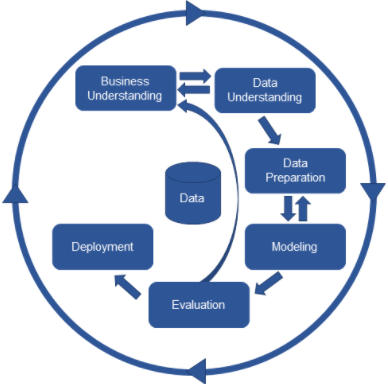
\includegraphics[width=9cm]{images/crisp.png}
			\caption{CRISP-DM Process}
			\label{fig:CRISP-DM}
		\end{center}
	\end{figure}
	
	\section{Structure of the Thesis}
	\label{section:structure} 
	The thesis will start by establishing a motivation and explaining the key objectives of the research, as well as explaining the research problem in Introduction part. Then thesis will review the existing literature in the Data Augmentation. From there on thesis will provide a brief overview of data and steps involved in data processing. In-depth analysis of data augmentation and evaluation will be provided in Modeling and Evaluation section. Finally, in conclusion section, the main findings, limitation, and recommendations will be discussed. 
	
	\section{Thesis Time Line}
	\label{section:Time Line} 
	The thesis will follow approximately the following time line.
	
	\begin{figure}[ht]
		\begin{center}
			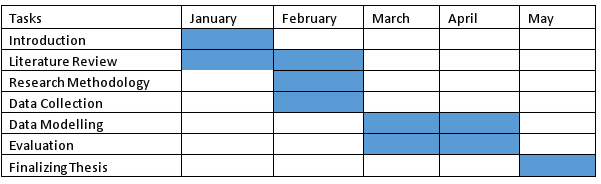
\includegraphics[width=9cm]{images/time.png}
			\caption{Thesis Time Line}
			\label{fig:Time Line}
		\end{center}
	\end{figure}
	
	\startchaprightThis is the text. And we shall rejoice.

	
	\bibliography{sources}
\end{document}
\grid
